\XtoCBlock{Sequencer}
\label{block:Sequencer}
\begin{figure}[H]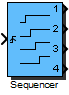
\includegraphics{Sequencer}\end{figure} 

\begin{XtoCtabular}{Inports}
Start & Start signal. Rising flank triggers sequence\tabularnewline
\hline
\end{XtoCtabular}


\begin{XtoCtabular}{Outports}
Out1 & Output \#1\tabularnewline
\hline
Out2 & Output \#2\tabularnewline
\hline
Out3 & Output \#3\tabularnewline
\hline
Out4 & Output \#4\tabularnewline
\hline
\end{XtoCtabular}

\begin{XtoCMaskParamTabular}{Mask Parameters}
\rowcolor[gray]{0.8}\textbf{Name} & \textbf{ID} & \textbf{Description}\tabularnewline\hline
Delay1 & 1 & Time delay for output 1\tabularnewline
\hline
Delay2 & 2 & Time delay for output 2\tabularnewline
\hline
Delay3 & 3 & Time delay for output 3\tabularnewline
\hline
Delay4 & 4 & Time delay for output 4\tabularnewline
\hline
ts\_fact & 5 & Multiplication factor of base sampling time (in integer format)\tabularnewline
\hline
\end{XtoCMaskParamTabular}

\subsubsection*{Description:}
Generation of time delayed (enable) sequence.

% include optional documentation file
\InputIfFileExists{\XcHomePath/Library/General/Doc/Sequencer_Info.tex}{\vspace{1ex}}{}

\subsubsection*{Implementations:}
\begin{tabular}{l l}
\textbf{FiP8} & 8 Bit Fixed Point Implementation\tabularnewline
\textbf{FiP16} & 16 Bit Fixed Point Implementation\tabularnewline
\textbf{FiP32} & 32 Bit Fixed Point Implementation\tabularnewline
\textbf{Float32} & 32 Bit Floating Point Implementation\tabularnewline
\textbf{Float64} & 64 Bit Floating Point Implementation\tabularnewline
\end{tabular}

\XtoCImplementation{FiP8}
\nopagebreak[0]

8 Bit Fixed Point Implementation

\begin{XtoCtabular}{Inports Data Type}
Start & int8\tabularnewline
\hline
\end{XtoCtabular}

\begin{XtoCtabular}{Outports Data Type}
Out1 & int8\tabularnewline
\hline
Out2 & int8\tabularnewline
\hline
Out3 & int8\tabularnewline
\hline
Out4 & int8\tabularnewline
\hline
\end{XtoCtabular}

\ifdefined \AddTestReports
\InputIfFileExists{\XcHomePath/Library/General/Doc/Test-Results/Test_Sequencer_FiP8.tex}{}{}
\fi
\XtoCImplementation{FiP16}
\nopagebreak[0]

16 Bit Fixed Point Implementation

\begin{XtoCtabular}{Inports Data Type}
Start & int16\tabularnewline
\hline
\end{XtoCtabular}

\begin{XtoCtabular}{Outports Data Type}
Out1 & int16\tabularnewline
\hline
Out2 & int16\tabularnewline
\hline
Out3 & int16\tabularnewline
\hline
Out4 & int16\tabularnewline
\hline
\end{XtoCtabular}

\ifdefined \AddTestReports
\InputIfFileExists{\XcHomePath/Library/General/Doc/Test-Results/Test_Sequencer_FiP16.tex}{}{}
\fi
\XtoCImplementation{FiP32}
\nopagebreak[0]

32 Bit Fixed Point Implementation

\begin{XtoCtabular}{Inports Data Type}
Start & int32\tabularnewline
\hline
\end{XtoCtabular}

\begin{XtoCtabular}{Outports Data Type}
Out1 & int32\tabularnewline
\hline
Out2 & int32\tabularnewline
\hline
Out3 & int32\tabularnewline
\hline
Out4 & int32\tabularnewline
\hline
\end{XtoCtabular}

\ifdefined \AddTestReports
\InputIfFileExists{\XcHomePath/Library/General/Doc/Test-Results/Test_Sequencer_FiP32.tex}{}{}
\fi
\XtoCImplementation{Float32}
\nopagebreak[0]

32 Bit Floating Point Implementation

\begin{XtoCtabular}{Inports Data Type}
Start & float32\tabularnewline
\hline
\end{XtoCtabular}

\begin{XtoCtabular}{Outports Data Type}
Out1 & float32\tabularnewline
\hline
Out2 & float32\tabularnewline
\hline
Out3 & float32\tabularnewline
\hline
Out4 & float32\tabularnewline
\hline
\end{XtoCtabular}

\ifdefined \AddTestReports
\InputIfFileExists{\XcHomePath/Library/General/Doc/Test-Results/Test_Sequencer_Float32.tex}{}{}
\fi
\XtoCImplementation{Float64}
\nopagebreak[0]

64 Bit Floating Point Implementation

\begin{XtoCtabular}{Inports Data Type}
Start & float64\tabularnewline
\hline
\end{XtoCtabular}

\begin{XtoCtabular}{Outports Data Type}
Out1 & float64\tabularnewline
\hline
Out2 & float64\tabularnewline
\hline
Out3 & float64\tabularnewline
\hline
Out4 & float64\tabularnewline
\hline
\end{XtoCtabular}

\ifdefined \AddTestReports
\InputIfFileExists{\XcHomePath/Library/General/Doc/Test-Results/Test_Sequencer_Float64.tex}{}{}
\fi
